\documentclass[9pt,twocolumn,twoside,]{pnas-new}

%% Some pieces required from the pandoc template
\providecommand{\tightlist}{%
  \setlength{\itemsep}{0pt}\setlength{\parskip}{0pt}}

% Use the lineno option to display guide line numbers if required.
% Note that the use of elements such as single-column equations
% may affect the guide line number alignment.


\usepackage[T1]{fontenc}
\usepackage[utf8]{inputenc}


\templatetype{pnasresearcharticle}  % Choose template

\title{Parsing medial prefrontal cortex: A joint meta-analytic and
graph-theoretic approach.}

\author[a,1,2]{Claudio A. Toro-Serey}
\author[a,1]{Joseph T. McGuire}

  \affil[a]{Boston University, Department of Psychological and Brain Sciences, 64
Commonwealth Ave., Boston, 02250}


% Please give the surname of the lead author for the running footer
\leadauthor{Toro-Serey}

% Please add here a significance statement to explain the relevance of your work
\significancestatement{Authors must submit a 120-word maximum statement about the significance
of their research paper written at a level understandable to an
undergraduate educated scientist outside their field of speciality. The
primary goal of the Significance Statement is to explain the relevance
of the work in broad context to a broad readership. The Significance
Statement appears in the paper itself and is required for all research
papers.}


\authorcontributions{Please provide details of author contributions here.}

\authordeclaration{Please declare any conflict of interest here.}

\equalauthors{\textsuperscript{} }

\correspondingauthor{\textsuperscript{} }

% Keywords are not mandatory, but authors are strongly encouraged to provide them. If provided, please include two to five keywords, separated by the pipe symbol, e.g:
 \keywords{  Networks |  DMN |  Valuation   }

\begin{abstract}
Valuation effects are consistently observed in medial prefrontal and
posterior cingulate cortex (mPFC and PCC). The spatial extent of these
effects is mostly indistinguishable from the default mode network (DMN)
in existing meta-analyses. However, little is known about how valuation
effects fit within the broader functional architecture of mPFC and PCC,
or whether that architecture is consistent or idiosyncratic across
individuals. Here we complement a meta-analysis with fMRI-based graph
theoretic approaches to subdivide mPFC and PCC at the single-subject
level. Our results suggest the functional topography of mPFC has
substantial variability across individuals. This highlights the
potential usefulness of estimating brain effects at the individual level
in this region, and points to limitations of aggregative methods such as
coordinate-based meta-analysis in determining whether valuation and DMN
effects emerge from common or separable brain systems. Our approach
shows promise in addressing this issue through future manipulations of
valuation.
\end{abstract}

\dates{This manuscript was compiled on \today}
\doi{\url{www.pnas.org/cgi/doi/10.1073/pnas.XXXXXXXXXX}}

\begin{document}

% Optional adjustment to line up main text (after abstract) of first page with line numbers, when using both lineno and twocolumn options.
% You should only change this length when you've finalised the article contents.
\verticaladjustment{-2pt}

\maketitle
\thispagestyle{firststyle}
\ifthenelse{\boolean{shortarticle}}{\ifthenelse{\boolean{singlecolumn}}{\abscontentformatted}{\abscontent}}{}

% If your first paragraph (i.e. with the \dropcap) contains a list environment (quote, quotation, theorem, definition, enumerate, itemize...), the line after the list may have some extra indentation. If this is the case, add \parshape=0 to the end of the list environment.

\acknow{Please include your acknowledgments here, set in a single paragraph.
Please do not include any acknowledgments in the Supporting Information,
or anywhere else in the manuscript.}

One of the main goals of human cognitive neuroscience is to be able to
prescribe function to brain regions, either in isolation or in their
communication with others. Among general regions of the brain, the
medial prefrontal cortex (mPFC, located in the midline frontal portion
of the brain) has been suggested to subserve the cognitive abilities
that differentiate humans from other animals (Barbas \& Garcia-Cabezas,
2016). Specifically, this region has been related to a variety of
functions, including decision making (Bartra, McGuire, \& Kable, 2013),
memory encoding (Shacter, Addis, \& Buckner, 2007), and default mode
deactivation (DMN) (Yeo et al., 2011). While much has been discovered
about this area in primates (Barbas \& Garcia-Cabezas, 2016), the lack
of direct measurements of neuronal activity makes this a tough area to
record in humans, one that nowadays relies mostly on functional MRI
(fMRI). Unfortunately, the mPFC is especially challenging to image, as
the oxygen-related signal recorded by fMRI is contaminated by the oxygen
in the sinuses (Logothetis, 2008). In addition, this area is subject to
more idiosyncratic cortical folding than any other region (Zilles,
Palomero- Gallagher, \& Amunts, 2013), thus adding a level of complexity
to the generalizable dissection of topographic functional roles within
mPFC.

Studies of valuation have consistently shown functional overlap with
DMN. Recent meta-analytic work has attempted to distinguish the brain
areas belonging to each by examining the locus of peak activity across
studies related to the behavioral features mentioned above (Bartra et
al., 2013; Acikalin, Gorgolewski, \& Poldrack, 2017). While this
approach offers valuable information, it is subject to the quality of
imaging in each study, as well as their corresponding differences in
tasks used to examine choice. In addition, recent findings suggest that
the functional topology of the brain is better understood by accounting
for organizational idosyncrasies (Braga and Buckner, 2018; Yeo et al.,
2018, Gordon et al., 2017, Gratton\ldots{}).

Given the shortcomings of study-specific and cross-study analyses
mentioned above, there is potential value in combining complementary
strengths from both approaches. While my lab is primarily interested in
the portion of mPFC dedicated to decision making, in order to bypass the
heterogeneity in behavioral tasks, it might be best to disentangle the
mPFC by focusing first on which of its sub-regions belong to
resting-state DMN, and which do not. The advantage lies in that (1) all
resting state scans are performed equally (the subject lies in the
scanner with their eyes open), and (2) there is a high quality resource
of resting state data provided by the Human Connectome Project. Focusing
on resting state data has been successful in determining a number of
neural phenomena, including disentangling auditory and visual attention
areas (Tobyne, Osher, Michalka, \& Somers, 2017).

This approach opens an opportunity to examine brain dynamics. For
example, a region's function might depend on its connectivity at any
given time with one brain community or another. An ever-growing trend in
human neuroimaging has been to apply network statistics to tackle these
functional challenges. One great advantage of network science is the
ability to characterize connectivity in a way that allows for
comparisons among individuals in a meaningful way (Garcia, Ashourvan,
Muldoon, Vettel, \& Bassett, 2018), thus letting us address the folding
idiosyncrasies mentioned above. Therefore, I propose to use some of the
statistics that we have learned in class to estimate intrinsic
functional subdivisions of the mPFC at the individual subject level.
Particularly, I would like to distinguish communities related to DMN
from non-DMN, so that we can generate more informed topographic targets
for future studies of decision making.

In this study, I try to address my question at 3 levels of granularity:
1) across the literature (meta-analysis), selecting a number of regions
of interest (ROI) that show significant overlap and specificity between
DMN and decision making; 2) full-brain connectivity of actual fMRI data,
using a pre-specified brain atlas; and 3) characterizing the
connectivity of surface vertices (small units of function that contain
oxygen-dependent neural information across time) for the regions
selected in step one. I performed the last two steps at an individual
subject level for 3 subjects, hoping to find some commonalities among
them. In this way, I attempted to extract functional topographical
information from topological network features.

\section*{Results}\label{results}
\addcontentsline{toc}{section}{Results}

\section*{Discussion}\label{discussion}
\addcontentsline{toc}{section}{Discussion}

\section*{Methods}\label{methods}
\addcontentsline{toc}{section}{Methods}

\section*{Results}\label{results-1}
\addcontentsline{toc}{section}{Results}

Please note that whilst this template provides a preview of the typeset
manuscript for submission, to help in this preparation, it will not
necessarily be the final publication layout. For more detailed
information please see the
\href{http://www.pnas.org/site/authors/format.xhtml}{PNAS Information
for Authors}.

\subsection*{Author Affiliations}\label{author-affiliations}
\addcontentsline{toc}{subsection}{Author Affiliations}

Include department, institution, and complete address, with the
ZIP/postal code, for each author. Use lower case letters to match
authors with institutions, as shown in the example. Authors with an
ORCID ID may supply this information at submission.

\subsection*{Submitting Manuscripts}\label{submitting-manuscripts}
\addcontentsline{toc}{subsection}{Submitting Manuscripts}

All authors must submit their articles at
\href{http://www.pnascentral.org/cgi-bin/main.plex}{PNAScentral}. If you
are using Overleaf to write your article, you can use the ``Submit to
PNAS'' option in the top bar of the editor window.

\subsection*{Format}\label{format}
\addcontentsline{toc}{subsection}{Format}

Many authors find it useful to organize their manuscripts with the
following order of sections; Title, Author Affiliation, Keywords,
Abstract, Significance Statement, Results, Discussion, Materials and
methods, Acknowledgments, and References. Other orders and headings are
permitted.

\subsection*{Manuscript Length}\label{manuscript-length}
\addcontentsline{toc}{subsection}{Manuscript Length}

PNAS generally uses a two-column format averaging 67 characters,
including spaces, per line. The maximum length of a Direct Submission
research article is six pages and a PNAS PLUS research article is ten
pages including all text, spaces, and the number of characters displaced
by figures, tables, and equations. When submitting tables, figures,
and/or equations in addition to text, keep the text for your manuscript
under 39,000 characters (including spaces) for Direct Submissions and
72,000 characters (including spaces) for PNAS PLUS.

\subsection*{References}\label{references}
\addcontentsline{toc}{subsection}{References}

References should be cited in numerical order as they appear in text;
this will be done automatically via bibtex, e.g. (1) and (2, 3). All
references, including for the SI, should be included in the main
manuscript file. References appearing in both sections should not be
duplicated. SI references included in tables should be included with the
main reference section.

\subsection*{Data Archival}\label{data-archival}
\addcontentsline{toc}{subsection}{Data Archival}

PNAS must be able to archive the data essential to a published article.
Where such archiving is not possible, deposition of data in public
databases, such as GenBank, ArrayExpress, Protein Data Bank, Unidata,
and others outlined in the Information for Authors, is acceptable.

\subsection*{Language-Editing Services}\label{language-editing-services}
\addcontentsline{toc}{subsection}{Language-Editing Services}

Prior to submission, authors who believe their manuscripts would benefit
from professional editing are encouraged to use a language-editing
service (see list at www.pnas.org/site/authors/language-editing.xhtml).
PNAS does not take responsibility for or endorse these services, and
their use has no bearing on acceptance of a manuscript for publication.

\begin{figure}
\centering
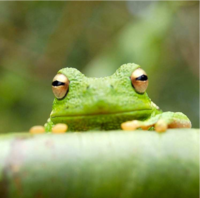
\includegraphics{frog.png}
\caption{Placeholder image of a frog with a long example caption to show
justification setting.{}}
\end{figure}

\subsection*{Digital Figures}\label{sec:figures}
\addcontentsline{toc}{subsection}{Digital Figures}

Only TIFF, EPS, and high-resolution PDF for Mac or PC are allowed for
figures that will appear in the main text, and images must be final
size. Authors may submit U3D or PRC files for 3D images; these must be
accompanied by 2D representations in TIFF, EPS, or high-resolution PDF
format. Color images must be in RGB (red, green, blue) mode. Include the
font files for any text.

Figures and Tables should be labelled and referenced in the standard way
using the \texttt{\textbackslash{}label\{\}} and
\texttt{\textbackslash{}ref\{\}} commands.

Figure \[fig:frog\] shows an example of how to insert a column-wide
figure. To insert a figure wider than one column, please use the
\texttt{\textbackslash{}begin\{figure*\}...\textbackslash{}end\{figure*\}}
environment. Figures wider than one column should be sized to 11.4 cm or
17.8 cm wide.

\subsection*{Single column equations}\label{single-column-equations}
\addcontentsline{toc}{subsection}{Single column equations}

Authors may use 1- or 2-column equations in their article, according to
their preference.

To allow an equation to span both columns, options are to use the
\texttt{\textbackslash{}begin\{figure*\}...\textbackslash{}end\{figure*\}}
environment mentioned above for figures, or to use the
\texttt{\textbackslash{}begin\{widetext\}...\textbackslash{}end\{widetext\}}
environment as shown in equation \[eqn:example\] below.

Please note that this option may run into problems with floats and
footnotes, as mentioned in the \href{http://texdoc.net/pkg/cuted}{cuted
package documentation}. In the case of problems with footnotes, it may
be possible to correct the situation using commands
\texttt{\textbackslash{}footnotemark} and
\texttt{\textbackslash{}footnotetext}.

\[\begin{aligned}
(x+y)^3&=(x+y)(x+y)^2\\
       &=(x+y)(x^2+2xy+y^2) \label{eqn:example} \\
       &=x^3+3x^2y+3xy^3+x^3. 
\end{aligned}\]

\subsection*{Supporting Information
(SI)}\label{supporting-information-si}
\addcontentsline{toc}{subsection}{Supporting Information (SI)}

The main text of the paper must stand on its own without the SI. Refer
to SI in the manuscript at an appropriate point in the text. Number
supporting figures and tables starting with S1, S2, etc. Authors are
limited to no more than 10 SI files, not including movie files. Authors
who place detailed materials and methods in SI must provide sufficient
detail in the main text methods to enable a reader to follow the logic
of the procedures and results and also must reference the online
methods. If a paper is fundamentally a study of a new method or
technique, then the methods must be described completely in the main
text. Because PNAS edits SI and composes it into a single PDF, authors
must provide the following file formats only.

\subsubsection*{SI Text}\label{si-text}
\addcontentsline{toc}{subsubsection}{SI Text}

Supply Word, RTF, or LaTeX files (LaTeX files must be accompanied by a
PDF with the same file name for visual reference).

\subsubsection*{SI Figures}\label{si-figures}
\addcontentsline{toc}{subsubsection}{SI Figures}

Provide a brief legend for each supporting figure after the supporting
text. Provide figure images in TIFF, EPS, high-resolution PDF, JPEG, or
GIF format; figures may not be embedded in manuscript text. When saving
TIFF files, use only LZW compression; do not use JPEG compression. Do
not save figure numbers, legends, or author names as part of the image.
Composite figures must be pre-assembled.

\subsubsection*{3D Figures}\label{d-figures}
\addcontentsline{toc}{subsubsection}{3D Figures}

Supply a composable U3D or PRC file so that it may be edited and
composed. Authors may submit a PDF file but please note it will be
published in raw format and will not be edited or composed.

\subsubsection*{SI Tables}\label{si-tables}
\addcontentsline{toc}{subsubsection}{SI Tables}

Supply Word, RTF, or LaTeX files (LaTeX files must be accompanied by a
PDF with the same file name for visual reference); include only one
table per file. Do not use tabs or spaces to separate columns in Word
tables.

\subsubsection*{SI Datasets}\label{si-datasets}
\addcontentsline{toc}{subsubsection}{SI Datasets}

Supply Excel (.xls), RTF, or PDF files. This file type will be published
in raw format and will not be edited or composed.

\subsubsection*{SI Movies}\label{si-movies}
\addcontentsline{toc}{subsubsection}{SI Movies}

Supply Audio Video Interleave (avi), Quicktime (mov), Windows Media
(wmv), animated GIF (gif), or MPEG files and submit a brief legend for
each movie in a Word or RTF file. All movies should be submitted at the
desired reproduction size and length. Movies should be no more than 10
MB in size.

\subsubsection*{Still images}\label{still-images}
\addcontentsline{toc}{subsubsection}{Still images}

Authors must provide a still image from each video file. Supply TIFF,
EPS, high-resolution PDF, JPEG, or GIF files.

\subsubsection*{Appendices}\label{appendices}
\addcontentsline{toc}{subsubsection}{Appendices}

PNAS prefers that authors submit individual source files to ensure
readability. If this is not possible, supply a single PDF file that
contains all of the SI associated with the paper. This file type will be
published in raw format and will not be edited or composed.

\showmatmethods
\showacknow
\pnasbreak

\hypertarget{refs}{}
\hypertarget{ref-belkin2002using}{}
1. Belkin M, Niyogi P (2002) Using manifold stucture for partially
labeled classification. \emph{Advances in Neural Information Processing
Systems}, pp 929--936.

\hypertarget{ref-berard1994embedding}{}
2. Bérard P, Besson G, Gallot S (1994) Embedding riemannian manifolds by
their heat kernel. \emph{Geometric \& Functional Analysis GAFA}
4(4):373--398.

\hypertarget{ref-coifman2005geometric}{}
3. Coifman RR, et al. (2005) Geometric diffusions as a tool for harmonic
analysis and structure definition of data: Diffusion maps.
\emph{Proceedings of the National Academy of Sciences of the United
States of America} 102(21):7426--7431.



% Bibliography
% \bibliography{pnas-sample}

\end{document}

